\documentclass[../template]{subfiles}

\begin{document}
\section{Minimum Spanning Tree}
\subsection{Algoritmo di Kruskal (Greedy)}
\begin{center}
    \begin{tikzpicture}[rotate=90]
        \Vertices[unit=2.3]{circle}{A,B,C,D,E}
        %\Edges(A,B,C,D,E)
        \Edge[color=red, label=$10$](A)(C)
        \Edge[label=$8$](A)(D)
        \Edge[color=red, label=$7$](D)(E)
        \Edge[color=red, label=$4$](A)(E)
        \Edge[color=red, label=$3$](B)(A)
        \Edge[label=$9$](B)(D)
        \Edge[label=$5$](B)(E)
        ;
    \end{tikzpicture}
\end{center}
\lstinputlisting{algorithms/mst_kruskal.py}
\subsubsection{Correttezza algoritmo di Kruskal}
\begin{enumerate}
    \item Supponiamo che per assurdo esista un MST, di peso inferiore a quello restituito dall'algoritmo greedy.
    \item Siccome i due alberi hanno il costo differente, hanno almeno un arco non in comune.
    \item Indicato con $e_h \in \{E_T - E_{T'}\}$ l'arco a peso minore appartenente all'albero restituito dall'algoritmo
        greedy, non appartenente all'albero preso per ipotesi $T'$.
    \item Dato che $T'$ è un MST, allora esiste un ciclo $C$ in $\{e_h\} \cup E_{T'}$ contenente $e_h$.
    \item Siccome anche $T$ è un albero, allora $C \cap E_{T} \neq \emptyset$, chiamiamo $e_r$ l'arco a peso minore,
        appartenente a $C \cap E_T - E_{T'}$.
    \item $w_{e_r} < w_{e_h}$, altrimenti l'algoritmo greedy applicato a $T$ avrebbe selezionato prima $e_h$ di $e_r$.
    \item Sostituendo in $T'$ l'arco $e_r$ con $e_h$, ottengo un nuovo albero di peso inferiore, contraddicendo l'ipotesi che
        $T'$ è l'albero di supporto a peso minore.
\end{enumerate}

\subsubsection{Analisi complessità}
$O(E \cdot \log (E))$, dovuta all'ordinamento degli archi in ordine di peso.
Il controllo dell'esistenza di cicli è effettuato in $O(1)$.

\subsection{Foresta di supporto}
Viene chiamata foresta di supporto di un grafo $G$ un grafo parziale $F = (V, E_F)$ privo di cicli. In particolare, un albero di
supporto è una foresta con una sola componente connessa.

\subsubsection{Teorema}
Indichiamo con $(V_1, E_1),\ldots ,(V_k, E_k)$ le componenti connesse di una foresta di supporto
$F = (V, E_F)$ del grafo $G$. Sia inoltre $(u, v)$ un arco a peso minimo tra quelli con un unico estremo
in $V_1$. Allora esiste almeno un albero di supporto a peso minimo appartenente a $\bigcup^k_{i=1} E_i$,
che contiene $(v, v)$.

\subsubsection{Dimostrazione}
Per assurdo, l'albero a peso minimo non contiene $(u, v)$. Ma aggiungendo $(u, v)$ a tale albero si forma un
ciclo contenente un altro arco $(u', v')$  con un solo estremo in $V_1$.
Se si toglie questo arco e si lascia $(u, v)$ si ottiene un albero di peso minore,
contraddicendo l'ipotesi.

\newpage
\subsection{Algoritmo di Prim (MST-1)}
Dijkstra
\begin{center}
    \begin{tikzpicture}[rotate=90]
        \Vertices[unit=2.3]{circle}{0,1,2,3,4}
        %\Edges(A,B,C,D,E)
        \Edge[color=red, label=$3$](0)(1)
        \Edge[label=$5$](0)(2)
        \Edge[label=$9$](0)(3)
        \Edge[label=$20$](0)(4)

        \Edge[color=red, label=$4$](1)(2)
        \Edge[label=$8$](1)(3)
        \Edge[color=red, label=$10$](1)(4)

        \Edge[label=$7$, color=red](2)(3)
        \Edge[label=$11$](2)(4)

        \Edge[label=$12$](3)(4)
        ;
    \end{tikzpicture}
\end{center}
\lstinputlisting{algorithms/mst_1.py}
% Lezione 4
\subsubsection{Correttezza MST-1}
Inizialmente abbiamo la foresta con $V_1 \equiv U = \{v_1\}, V_i = \{v_i\} \quad i=2\ldots n$, con tutti gli $E_i = \emptyset$.

Alla prima iterazione si inserisce l'arco $(V_i, v_{j_1})$, $j_1 \neq 1$, a peso minimo tra quelli con un solo estremo in $U \equiv V_1$
e quindi, per il teorema visto al paragrafo della foresta di supporto, tale arco farà parte dell'albero di supporto a peso minimo
tra tutti i possibili alberi di supporto.

Con l'aggiunta di questo arco, le due componenti connesse $(V_1, E_1)$ e $(V_{j_1}, E_{j_1})$ si fondono in un'unica componente
connessa con nodi $U = \{v_i, v_{j_1}\}$ e l'insieme di archi $E_T = \{(v_1, v_{j_1})\}$, mentre le altre componenti connesse non cambiano.
Abbiamo cioè che le componenti connesse
\[(U, E_T), \quad (V_i, \emptyset) i \in \{2,\ldots n\} - \{j_1\}\]

Alla seconda iterazione andiamo a selezionare il nodo $v_{j_2}$ e il relativo arco $( v_{j_2}, c(v_{j_2}))$ con il peso minimo
tra tutti quelli con un solo estremo in $U$.
In base al teorema, l'arco $(v_{j_2}, c(v_{j_2}))$ farà parte di un albero di supporto a peso minimo tra tutti quelli che contengono
l'unione di tutti gli archi delle componenti connesse, che si riduce ad $E_T$.

Effettuiamo lo stesso ragionamento per tutti gli $n$ ottenendo l'albero di supporto a peso minimo.
\subsubsection{Complessità dell'algoritmo}
Il numero di operazioni richiesto è pari a $O(V^2)$ dovuta al ciclo eseguito $V$ volte ($O(V)$) e la ricerca del minimo in tempo lineare.

\subsubsection{Confronto con algoritmo di Kruskal}
Anche se risulta essere peggiore rispetto all'algoritmo di greedy Kruskal, è possibile dimostrare che, in caso di grafi densi
ha una complessità ottima.
Infatti per tali grafi non possiamo aspettarci di fare meglio di $O(V^2)$: la sola operazione di lettura dei pesi
degli archi richiede $O(V^2)$.

\subsection{Algoritmo Borůkova (MST-2)}
\lstinputlisting{algorithms/mst_2.py}
\subsubsection{Dimostrazione correttezza}
Lasciata per esercizio, si basa sul teorema della foresta.
\textit{"Tutti gli archi shortest aggiunti ad una certa iterazione, sono tutti archi
che fanno parte ad un albero di supporto ottimo, tra tutti i possibili
alberi di supporto."}

\subsubsection{Complessità algoritmo}
$O(E \cdot \log_2 (V))$ derivato dal costo dell'iterazione su tutti gli archi
$O(E)$, eseguita un numero massimo di $\log(|V|)$ volte.

Inizialmente il numero di componenti connesse è pari al numero di nodi.
Sicuramente ad ogni iterazione, il numero di componenti connesse viene
almeno dimezzato. Per cui, il primo ciclo viene eseguito al più $\log(|V|)$
volte.

Per grafi densi con $|E| = O(|V|^2)$ questa complessità
è peggiore di quella di MST-1, ma se il numero di archi scende sotto l'ordine $O(|V|^2/log(|V|))$ l'algoritmo MST-2 ha prestazioni migliori.

\subsection{Note}
Questi tre algoritmi appena visti sono tutti e tre algoritmi costruttivi, senza revisione delle decisioni passate.
\end{document}
